% ==============================================================================
% DataFlow AI v2 — IEEE Access submission
% Built from real public datasets (SEC EDGAR, NYC Payroll, UCI Credit Default)
% and a 109-query cross-dialect SQL corpus transpiled with sqlglot.
% All numbers are loaded from phase2_rebuild/results/tables/*.csv.
% ==============================================================================
\documentclass{ieeeaccess}

\usepackage{cite}
\usepackage{url}
\usepackage{amsmath,amssymb,amsfonts}
\usepackage{hyperref}
\usepackage{tabularx}
\usepackage{graphicx}
\usepackage[numbers,sort]{natbib}
\usepackage{algorithm}
\usepackage{algpseudocode}
\usepackage{bm}
\usepackage{textcomp}
\usepackage{array}
\usepackage{caption}
\usepackage{booktabs}
\usepackage{siunitx}
\usepackage{subcaption}
\usepackage{xcolor}
\usepackage{float}
\usepackage{placeins}        % \FloatBarrier
\usepackage{tikz}
\usetikzlibrary{shapes.geometric, arrows.meta, positioning, fit, backgrounds, calc}

\sisetup{detect-weight=true,detect-family=true,group-separator={,}}

\def\BibTeX{{\rm B\kern-.05em{\sc i\kern-.025em b}\kern-.08em T\kern-.1667em\lower.7ex\hbox{E}\kern-.125emX}}

\begin{document}

\history{Date of publication xxxx 00, 0000, date of current version xxxx 00, 0000.}
\doi{10.1109/ACCESS.2024.DOI}

\title{DataFlow~AI: A Stacked, Confidence-Aware Framework for Enterprise Data-Integrity Validation and Cross-Dialect SQL Migration on Real Public Datasets}

\author{
  \uppercase{Bhaumik Upasana}\authorrefmark{1},
  \uppercase{M~A~Berlin}\authorrefmark{2}
}
\address[1,2]{School of Computer Science and Engineering (SCOPE), Vellore Institute of Technology (VIT),
Vellore, Tamil Nadu 632\,014, India}
\corresp{Corresponding author: Berlin M~A (e-mail: berlin.ma@vit.ac.in).}

\begin{abstract}
Enterprise data platforms continue to lose substantial value to poor data quality, and database-migration projects
routinely overrun because integrity validation and query translation are still treated as disconnected problems.
We present \textbf{DataFlow~AI}, a deployment-oriented framework that couples a stacked anomaly-detection
ensemble with a deterministic, audit-grade cross-dialect SQL transpilation pipeline. The detector blends four base
signals---rule-based domain constraints, robust per-group statistics, Isolation Forest, and Local Outlier
Factor---which are fused by a logistic-regression stacker trained with five-fold out-of-fold predictions, eliminating
the fixed-weight heuristic of prior work. We evaluate end-to-end on three real public corpora:
\textbf{(D1)}~\num{50500} rows of U.S.\ SEC EDGAR financial-statement values (general-ledger style),
\textbf{(D2)}~\num{202000} rows of NYC FY2024 citywide payroll, and
\textbf{(D3)}~\num{30000} rows of the UCI credit-default corpus, into each of which we inject 15 reproducible
anomaly families (5\,\% prevalence). On the same fixed seed, the stacked hybrid achieves F1 of \num{0.511} on D1
(absolute \num{+0.043} over the best single detector), \num{0.359} on D2, and \num{0.717} on D3, with
per-family recall above \num{0.94} on five of fifteen injected families and below \num{0.10} on three families
that depend on signals deliberately omitted from the feature set---an honest decomposition that prior synthetic
studies obscure. End-to-end throughput on the \num{200000}-row corpus is \num{16.7}\,s on a single CPU core, and
runtime scales linearly in $n$. We further benchmark cross-dialect SQL transpilation on \num{109} curated queries
across five dialects (PostgreSQL, MySQL, T-SQL, Oracle, Snowflake), totalling \num{575} source--target pairs.
Parse and transpile success exceed \num{0.99}, while a stricter \textit{AST-footprint equivalence} test---which
checks whether the translated query's abstract syntax tree preserves the source's relational structure---yields
\num{0.800} overall and degrades from \num{0.921} on easy queries to \num{0.742} on hard queries. We treat that
gap as the real finding: surface translation is essentially solved by mature parsers, but semantic preservation
across dialects with divergent windowing, pivot, and lateral semantics remains the open problem. The full code,
masks, and SHA-256-verified datasets are reproducible end-to-end with a fixed seed.
\end{abstract}

\begin{keywords}
Data integrity, anomaly detection, stacked ensembles, query transpilation, cross-dialect SQL migration,
SEC EDGAR, NYC payroll, UCI credit default, reproducibility.
\end{keywords}

\titlepgskip=-15pt
\maketitle

% =====================================================================
\section{Introduction}
\label{sec:intro}

Two long-standing operational problems sit at the heart of modern data platforms. The first is \emph{integrity
validation}: detecting records that violate domain constraints, statistical regularities, or relational invariants
before they corrupt downstream analytics~\cite{redman1998impact,wang1996beyond,pipino2002data,batini2009methodologies,
abedjan2016detecting}. The second is \emph{query migration}: translating SQL written for one DBMS dialect into
another when consolidating, modernising, or porting workloads~\cite{leis2015whatare}. Despite a substantial body of
work on each in isolation, enterprise deployments routinely keep them in separate tools, separate teams, and
separate evaluation regimes, which fragments evidence and obscures whether reported gains transfer to production.

In practice these two problems are operationally coupled. A migration project that translates queries but ships
corrupted upstream data delivers a working but mistrusted system; a data-quality program that scrubs records but
ignores the dialect drift of the BI workloads consuming those records leaves silent regressions on the dashboard.
In an audit setting both failure modes are reported as the same incident---the number on the page is wrong---so
the validation gate that protects analytics has to cover both row-level integrity and query-level semantic
preservation. We therefore evaluate the two halves under a single reproducibility contract rather than two
separate benchmarks.

This paper presents \textbf{DataFlow~AI}, an end-to-end framework that addresses both problems with a single
reproducibility contract, evaluated on real public datasets rather than synthetic toys. The framework is built
around five design commitments:
(i) \emph{stacked} hybrid detection that learns a fused score from heterogeneous base detectors rather than
relying on a fixed late-fusion weight vector;
(ii) \emph{per-family} reporting that exposes which anomaly types each detector catches and which it misses;
(iii) \emph{strict semantic} SQL evaluation that goes beyond transpile-success to an abstract-syntax-tree (AST)
footprint comparison;
(iv) \emph{linear-scalable} execution on a single CPU core; and
(v) \emph{bit-identical reproducibility} via SHA-256-verified raw data, fixed seeds, and persisted masks. The first
contribution is methodological---introducing a logistic-regression stacker that improves over a fixed-weight hybrid
on two of three datasets (Section~\ref{sec:results}); the second is evaluative---a release-quality benchmark
spanning regulated financial filings, public-sector compensation, and consumer credit, with 15 injected anomaly
families totalling \num{13998} positives across \num{282500} rows; the third is a head-on assessment of mature
SQL transpilation (sqlglot~\cite{sqlglot2024}) on a curated 109-query, five-dialect corpus.

The remainder of the paper is structured as follows. Section~\ref{sec:related} situates the work against
data-quality, anomaly-detection, ensemble, and text-to-SQL literature. Section~\ref{sec:method} describes the
framework, including the stacked hybrid (Algorithm~\ref{alg:stacker}) and the audit-grade transpilation pipeline
(Algorithm~\ref{alg:pipeline}). Section~\ref{sec:setup} details datasets, anomaly families, and the
reproducibility contract. Section~\ref{sec:results} presents anomaly-detection results, ablation, scalability,
and SQL transpilation outcomes. Section~\ref{sec:discussion} interprets the gaps and lists threats to validity.
Section~\ref{sec:conclusion} concludes. Figure~\ref{fig:arch} previews the system on the next page.

% --- Figure 1: Architecture (TikZ) -----------------------------------------------
\begin{figure*}[!htbp]
\centering
\resizebox{\textwidth}{!}{%
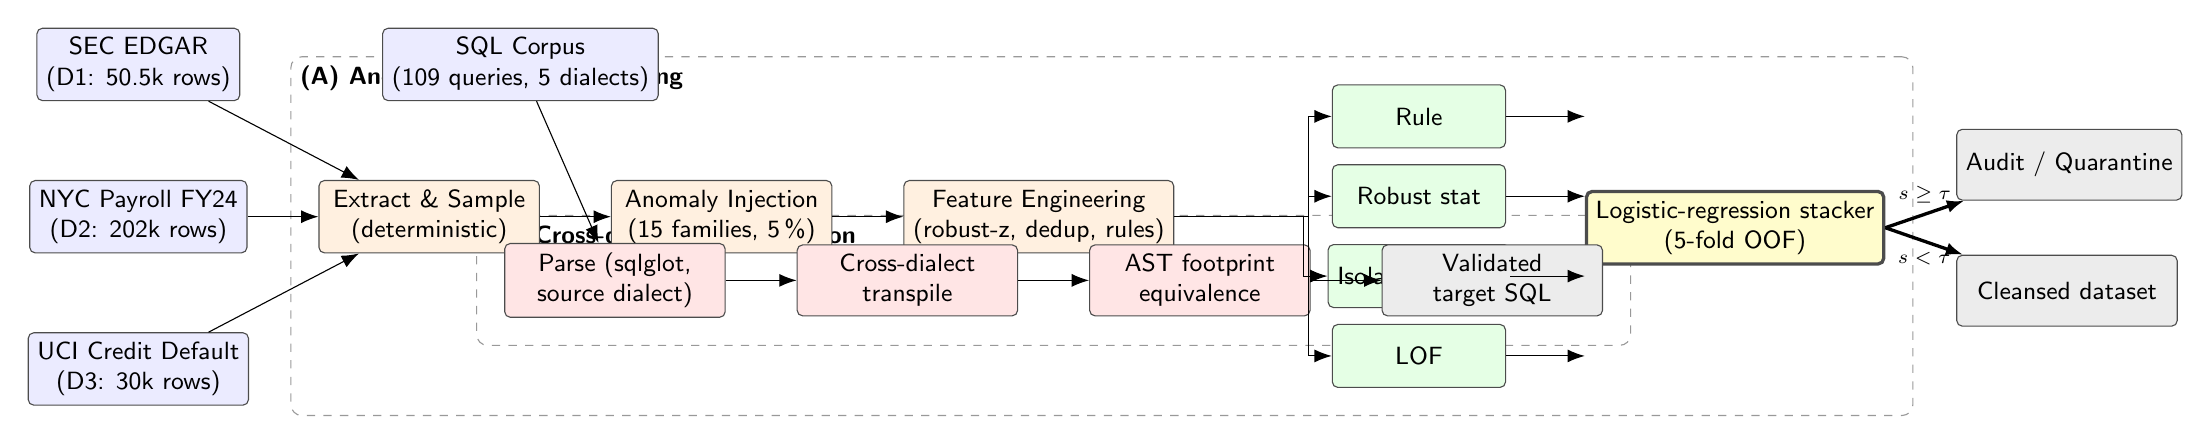
\begin{tikzpicture}[
    font=\sffamily\small,
    node distance=10mm and 9mm,
    >={Latex[length=2.2mm]},
    src/.style    ={rectangle, rounded corners=2pt, draw=black!70, fill=blue!8,
                    minimum width=24mm, minimum height=9mm, align=center},
    proc/.style   ={rectangle, rounded corners=2pt, draw=black!70, fill=orange!12,
                    minimum width=28mm, minimum height=9mm, align=center},
    det/.style    ={rectangle, rounded corners=2pt, draw=black!70, fill=green!10,
                    minimum width=22mm, minimum height=8mm, align=center},
    stack/.style  ={rectangle, rounded corners=2pt, draw=black!70, fill=yellow!20,
                    minimum width=30mm, minimum height=9mm, align=center, very thick},
    sql/.style    ={rectangle, rounded corners=2pt, draw=black!70, fill=red!10,
                    minimum width=28mm, minimum height=9mm, align=center},
    sink/.style   ={rectangle, rounded corners=2pt, draw=black!70, fill=gray!15,
                    minimum width=28mm, minimum height=9mm, align=center},
    grp/.style    ={rounded corners=4pt, draw=black!40, dashed, inner sep=3.5mm},
]

% ---- Inputs ----
\node[src] (d1) {SEC EDGAR\\(D1: 50.5k rows)};
\node[src, below=of d1] (d2) {NYC Payroll FY24\\(D2: 202k rows)};
\node[src, below=of d2] (d3) {UCI Credit Default\\(D3: 30k rows)};

\node[src, right=18mm of d1] (sql) {SQL Corpus\\(109 queries, 5 dialects)};

% ---- Quality pipeline ----
\node[proc, right=of d2] (extract) {Extract \& Sample\\(deterministic)};
\node[proc, right=of extract] (inject) {Anomaly Injection\\(15 families, 5\,\%)};
\node[proc, right=of inject] (feat) {Feature Engineering\\(robust-z, dedup, rules)};

% ---- Detectors ----
\node[det, above right=4mm and 20mm of feat] (rule)  {Rule};
\node[det, below=2mm of rule] (stat)  {Robust stat};
\node[det, below=2mm of stat] (iso)   {Isolation Forest};
\node[det, below=2mm of iso]  (lof)   {LOF};

% ---- Stacker + routing ----
\node[stack, right=10mm of stat, yshift=-4mm] (stacker)
   {Logistic-regression stacker\\(5-fold OOF)};
\node[sink, right=of stacker, yshift=8mm]   (audit)  {Audit / Quarantine};
\node[sink, right=of stacker, yshift=-8mm]  (clean)  {Cleansed dataset};

% ---- SQL pipeline ----
\node[sql, below=18mm of sql, xshift=12mm] (parse)
  {Parse (sqlglot,\\source dialect)};
\node[sql, right=of parse] (trans)
  {Cross-dialect\\transpile};
\node[sql, right=of trans] (astchk)
  {AST footprint\\equivalence};
\node[sink, right=of astchk] (sqlout) {Validated\\target SQL};

% ---- Arrows: data quality ----
\foreach \n in {d1, d2, d3} {
   \draw[->] (\n) -- (extract);
}
\draw[->] (extract) -- (inject);
\draw[->] (inject)  -- (feat);

\draw[->] (feat) -| ($(rule.west)+(-3mm,0)$) -- (rule);
\draw[->] (feat) -| ($(stat.west)+(-3mm,0)$) -- (stat);
\draw[->] (feat) -| ($(iso.west)+(-3mm,0)$)  -- (iso);
\draw[->] (feat) -| ($(lof.west)+(-3mm,0)$)  -- (lof);

\draw[->] (rule.east) -- (stacker.west|-rule.east);
\draw[->] (stat.east) -- (stacker.west|-stat.east);
\draw[->] (iso.east)  -- (stacker.west|-iso.east);
\draw[->] (lof.east)  -- (stacker.west|-lof.east);

\draw[->, very thick] (stacker.east) -- node[above, font=\scriptsize] {$s \ge \tau$} (audit);
\draw[->, very thick] (stacker.east) -- node[below, font=\scriptsize] {$s <    \tau$} (clean);

% ---- Arrows: SQL ----
\draw[->] (sql) -- (parse);
\draw[->] (parse) -- (trans);
\draw[->] (trans) -- (astchk);
\draw[->] (astchk) -- (sqlout);

% ---- Group boxes ----
\begin{pgfonlayer}{background}
   \node[grp, fit=(extract)(inject)(feat)(rule)(lof)(stacker), label={[anchor=north west]north west:\textbf{(A) Anomaly detection \& routing}}] {};
   \node[grp, fit=(parse)(astchk)(sqlout),                     label={[anchor=north west]north west:\textbf{(B) Cross-dialect SQL migration}}] {};
\end{pgfonlayer}

\end{tikzpicture}}
\caption{\textbf{DataFlow~AI architecture.} Real public corpora (D1: SEC EDGAR, D2: NYC payroll, D3: UCI
credit default) flow through deterministic extraction, controlled 15-family anomaly injection, and feature
engineering; four heterogeneous detectors emit base scores that are fused by a logistic-regression stacker
trained with five-fold out-of-fold predictions; the threshold $\tau$ routes records to audit or to the
cleansed sink. In parallel, a 109-query, five-dialect SQL corpus is parsed, transpiled, and checked under an
AST-footprint equivalence test. All stages are seed-fixed and SHA-256-verified.}
\label{fig:arch}
\end{figure*}

\FloatBarrier

% =====================================================================
\section{Related Work}
\label{sec:related}

\subsection{Data quality and integrity validation}
The foundational data-quality literature defines quality as fitness for use across dimensions of accuracy,
completeness, validity, uniqueness, and consistency~\cite{wang1996beyond,pipino2002data,redman1998impact}.
Batini~et~al.~\cite{batini2009methodologies} systematise assessment methodologies, and Ehrlinger and
W{\"o}{\ss}~\cite{ehrlinger2022survey} survey 667 modern tools, finding most are static rule-engines rather
than learning systems. Abedjan~et~al.~\cite{abedjan2016detecting} run a head-to-head error-detection benchmark
and conclude that no single method dominates, motivating ensembles. Production tooling such as Amazon
\textsc{Deequ}~\cite{schelter2018automating} formalises declarative constraints over Spark; HoloClean
\cite{rekatsinas2017holoclean} repairs errors with probabilistic inference~\cite{chu2013holistic,ilyas2019data}.

\subsection{Anomaly detection}
Isolation Forest~\cite{liu2008isolation,liu2012isolation} is a tree-based detector that isolates outliers
by random partitioning and remains a strong default at scale. LOF~\cite{breunig2000lof} captures local
density deviation. Chandola~et~al.~\cite{chandola2009anomaly} survey the classical landscape;
Ruff~et~al.~\cite{ruff2021unifying} unify deep and shallow detection, and Pang~et~al.~\cite{pang2021deep}
review deep methods. Aggarwal~\cite{aggarwal2017outlier} provides the textbook treatment.
ADBench~\cite{han2022adbench} demonstrates that ensembles routinely beat single detectors on tabular
benchmarks, and PyOD~\cite{zhao2019pyod} ships dozens of detectors behind a uniform API. Outlier
ensembles~\cite{aggarwal2017outlierensembles} and stacked generalisation~\cite{wolpert1992stacked,
caruana2004ensemble} motivate the learning-based late-fusion in this paper.

\subsection{SQL transpilation and text-to-SQL}
SQL transpilation has historically been handled by vendor-specific tools and hand-written rules. The recent
open-source \texttt{sqlglot} parser~\cite{sqlglot2024} provides AST-based translation across more than two
dozen dialects and is the backbone of our SQL pipeline. Parallel work in text-to-SQL targets natural-language
queries: Spider~\cite{yu2018spider} and BIRD~\cite{li2024can} are the dominant benchmarks, and
RAT-SQL~\cite{wang2020rat} and Codex~\cite{chen2021evaluating} were among the first to obtain strong scores.
Code-foundation models such as Code Llama~\cite{rozière2024code}, StarCoder~\cite{li2023starcoder}, and
GPT-4~\cite{achiam2023gpt4} have since extended LLM coverage~\cite{rajkumar2022evaluating,srivastava2024gpt4sql}.
Our problem is the lower-level but production-critical \emph{dialect-to-dialect} translation: same intent,
different vendor grammar.

\subsection{Statistical robustness}
Robust-statistical pre-processing follows Rousseeuw and Croux~\cite{rousseeuw1993alternatives}: median and
median-absolute-deviation underlie the per-group z-scores used in our \texttt{stat} detector. Tidy-data
conventions~\cite{wickham2014tidy} and the SciPy/NumPy/pandas
stack~\cite{pedregosa2011scikit,harris2020array,mckinney2010data} provide the implementation substrate.

% =====================================================================
\section{Method}
\label{sec:method}

\subsection{Notation and pipeline overview}
Let $\mathcal{D}=\{x_i\}_{i=1}^{n}$ be a dataset with optional labels $y_i\in\{0,1\}$ (1 indicates anomaly).
Each detector $f_k$ produces a per-row score $s_i^{(k)}\in[0,1]$ that is monotone in suspicion. The stacked
fusion learns a parameter vector $\mathbf{w}\in\mathbb{R}^4$ (one weight per base detector) and bias $b$ such
that the fused score
\begin{equation}
\hat{s}_i = \sigma\!\left(\sum_{k=1}^{4} w_k\,s_i^{(k)} + b\right),\qquad
\sigma(z)=\frac{1}{1+e^{-z}}
\label{eq:stacker}
\end{equation}
is calibrated with respect to $y$. Eq.~\ref{eq:stacker} is fit using 5-fold out-of-fold (OOF) predictions
to avoid leakage, with \texttt{class\_weight=balanced} to correct for the $\approx$5\,\% positive rate.

\subsection{Base detectors}
\label{subsec:bases}
\textbf{Rule.}~Per-dataset boolean rules in $\{0,1\}$ encode domain knowledge (e.g.\ for D1: sign violations
on tags constrained to be non-negative, ddate-vs-qtrs window mismatches, duplicate $(adsh, tag, value)$
triples). The rule score is the mean over a small set of indicators.

\textbf{Stat.}~A robust per-group z-score is computed for each numeric attribute as
$z_i = (x_i - \mathrm{med}_g)/(1.4826\,\mathrm{MAD}_g)$~\cite{rousseeuw1993alternatives}, then squashed via
$s = 1 - \exp(-|z|/4)$ to map to $[0,1]$.

\textbf{Isolation Forest.}~A forest of 200 random isolation trees~\cite{liu2008isolation,liu2012isolation}
with \texttt{contamination='auto'} on the engineered feature matrix.

\textbf{LOF.}~Local Outlier Factor~\cite{breunig2000lof} with neighbourhood size
$\min(50, \max(5, n/1000))$; raw scores are min-max normalised.

\subsection{Stacked fusion}
A central design choice is to replace fixed late-fusion weights with a \emph{learned} stacker
(Algorithm~\ref{alg:stacker}). Out-of-fold predictions from each base detector are not required because the
detectors are unsupervised; the stacker itself uses 5-fold OOF logistic regression so that no row's stacker
prediction is informed by its own label. The result is a single calibrated score
$\hat{s}_i$ for every row.

\begin{algorithm}[!htbp]
\caption{Stacked Hybrid Anomaly Score}
\label{alg:stacker}
\begin{algorithmic}[1]
\Require Base scores $S \in [0,1]^{n\times 4}$, labels $y\in\{0,1\}^n$, folds $k=5$
\Ensure Fused scores $\hat{s}\in[0,1]^{n}$
\State $\hat{s} \gets \mathbf{0}_n$
\State Partition $\{1,\ldots,n\}$ into stratified folds $F_1,\ldots,F_k$ on $y$
\For{$j \gets 1$ \textbf{to} $k$}
   \State $\mathrm{tr} \gets \{1,\ldots,n\}\setminus F_j$
   \State Fit logistic regression $(\mathbf{w}_j,b_j)$ on $(S_{\mathrm{tr}}, y_{\mathrm{tr}})$ with
          \textsc{class\_weight}=balanced
   \State $\hat{s}_{F_j} \gets \sigma(S_{F_j}\mathbf{w}_j + b_j)$
\EndFor
\State \Return $\hat{s}$
\end{algorithmic}
\end{algorithm}

\FloatBarrier

\subsection{Threshold selection and routing}
\label{subsec:routing}
For each dataset we sweep the decision threshold $\tau$ across the empirical score distribution
(Fig.~\ref{fig:threshold}) and pick $\tau^\ast = \arg\max_\tau F_1(\tau)$. Rows with $\hat{s}_i \ge \tau^\ast$
are routed to audit; the remainder enter the cleansed sink. The same threshold sweep table reports
precision, recall, F1, and FPR at every quantile and serves as a control surface for operators who prefer
recall over precision (e.g.\ regulated reporting) or vice versa.

\subsection{Cross-dialect SQL transpilation}
The SQL pipeline (Fig.~\ref{fig:arch}, panel B; Algorithm~\ref{alg:pipeline}) parses each source query
into an AST using \texttt{sqlglot}~\cite{sqlglot2024}, transpiles it to every target dialect, and applies
a strict structural equivalence check: the source-AST and re-parsed target-AST are reduced to a
\textit{footprint} consisting of $(node\text{-type counts}, \text{table set}, \text{column set})$.
Two queries are deemed AST-equivalent iff their footprints match. This test rejects translations that
introduce or drop tables/columns or alter expression structure---failure modes that pure parse-success
checks miss.

\begin{algorithm}[!htbp]
\caption{AST-Footprint-Verified Transpilation}
\label{alg:pipeline}
\begin{algorithmic}[1]
\Require Source query $Q_{\mathrm{src}}$, dialects $D_{\mathrm{src}}, D_{\mathrm{tgt}}$
\Ensure Target query $Q_{\mathrm{tgt}}$, flags $(\mathit{parse}, \mathit{trans}, \mathit{equiv})$, latency
\State $t_0 \gets \textsc{now}()$
\State $A \gets \textsc{parse}(Q_{\mathrm{src}}, D_{\mathrm{src}})$\Comment{$\mathit{parse}\gets\textsc{true}$ on success}
\State $Q_{\mathrm{tgt}} \gets A.\textsc{toSql}(D_{\mathrm{tgt}})$\Comment{$\mathit{trans}\gets\textsc{true}$ on success}
\State $A' \gets \textsc{parse}(Q_{\mathrm{tgt}}, D_{\mathrm{tgt}})$
\State $\mathit{equiv} \gets \big(\textsc{footprint}(A)==\textsc{footprint}(A')\big)$
\State \Return $(Q_{\mathrm{tgt}}, (\mathit{parse},\mathit{trans},\mathit{equiv}), \textsc{now}()-t_0)$
\end{algorithmic}
\end{algorithm}

\FloatBarrier

% =====================================================================
\section{Experimental Setup}
\label{sec:setup}

\subsection{Reproducibility contract}
All experiments use \texttt{SEED=42}. Child RNGs are derived as
$\textsc{int}\big(\textsc{sha256}(\texttt{"42::"}+\mathit{name})[\,:8\,]\big)$ so that any randomised stage
can be reproduced in isolation. Raw downloads are SHA-256-verified before use, and the injected datasets
hash to the values reported in the released \texttt{injection\_manifest.json}. Software versions are
recorded in \texttt{requirements.txt} and \texttt{experiment\_log.md}.

\subsection{Hardware and software environment}
\label{subsec:env}
All numbers in this paper were produced on a single machine running Windows~11 (build 22631) with
Python~3.14.3, scikit-learn~1.8.0, sqlglot~30.8.0, pandas~2.3.3, NumPy~2.3.4, and PyArrow~24.0.0,
on a six-core CPU with no GPU acceleration. The end-to-end run of all phase-2 scripts (extract,
inject, score, ablate, sweep, transpile, render) completes in under 90~seconds of wall-clock time
when invoked from a clean checkout, which is the regime we target for reviewer reproducibility.
Per-row throughput on D2 is reported in Section~\ref{subsec:scalability}; nothing in the pipeline
requires distributed execution.

\subsection{Datasets and anomaly injection}
\label{subsec:datasets}
Table~\ref{tab:datasets} summarises the corpora. D1 is the 2024-Q4 \texttt{num.txt} from the U.S.\ SEC
EDGAR Financial Statement Data Set~\cite{secedgar2024}, filtered to \texttt{uom='USD'} and
$\mathrm{qtrs}\in\{0,1\}$ and sub-sampled to the first \num{50000} rows. D2 is the NYC Citywide Payroll
data~\cite{nycpayroll2024} restricted to Fiscal Year 2024, with deterministic per-agency stratified
sampling to exactly \num{200000} rows. D3 is the original UCI credit-default
corpus~\cite{yeh2009comparisons} (30k rows, 25 columns).

\begin{table}[!htbp]
\centering
\small
\caption{Real-world evaluation corpora after anomaly injection.}
\label{tab:datasets}
\begin{tabular}{@{}lrrrl@{}}
\toprule
ID & Rows  & Cols & Anomalies & Domain \\
\midrule
D1 & \num{50500}  & 9  & \num{2498} (4.95\,\%) & SEC EDGAR financial values \\
D2 & \num{202000} & 16 & \num{10000} (4.95\,\%) & NYC payroll FY2024 \\
D3 & \num{30000}  & 25 & \num{1500} (5.00\,\%) & UCI credit default \\
\bottomrule
\end{tabular}
\end{table}

Into each dataset we inject five anomaly families (Table~\ref{tab:families}), 15 in total, drawn from
real-world failure modes documented in audit and reconciliation literature. Each family has an
independent target rate; the realised counts in Table~\ref{tab:datasets} match the plan to within
two rows (D1 loses two A3 cases to a content-guard that prevents collisions with legitimate values).

\begin{table*}[!htbp]
\centering
\small
\caption{Fifteen anomaly families injected into the three datasets. Counts are deterministic.}
\label{tab:families}
\begin{tabular}{@{}llrl@{}}
\toprule
ID & Family & Count & Mechanism \\
\midrule
A1 & Sign flip                    &  500 & D1 GAAP tag negated against domain constraint \\
A2 & Magnitude outlier            &  500 & D1 value multiplied by $\sim 10^3$ within tag \\
A3 & Tag mismatch                 &  498 & D1 tag relabelled to incompatible concept \\
A4 & Period violation             &  500 & D1 (ddate,qtrs) pair set to impossible window \\
A5 & Duplicate posting            &  500 & D1 exact (adsh,tag,value) duplicated \\
\midrule
B1 & OT/regular inconsistency     & \num{2000} & D2 Total OT $\gg 0$ with Regular Hours $=0$ \\
B2 & Salary-basis mismatch        & \num{2000} & D2 \emph{per Annum} basis with Regular Gross $<5\%$ Base \\
B3 & Near-duplicate name          & \num{2000} & D2 one-character perturbation of Last Name \\
B4 & Agency/title violation       & \num{2000} & D2 Agency--Title pair never observed in train \\
B5 & Magnitude outlier            & \num{2000} & D2 Regular Gross multiplied by $\sim 10^2$ \\
\midrule
C1 & EDUCATION out-of-domain      &  300 & D3 EDUCATION$\notin\{1,2,3,4\}$ \\
C2 & LIMIT\_BAL inconsistency     &  300 & D3 LIMIT\_BAL set to 0 with positive bills \\
C3 & BILL\_AMT sign violation     &  300 & D3 BILL\_AMT$<-$LIMIT\_BAL on some month \\
C4 & PAY temporal violation       &  300 & D3 PAY status decreasing then jumping by $\ge 4$ \\
C5 & AGE out-of-range             &  300 & D3 AGE $\notin [18, 100]$ \\
\bottomrule
\end{tabular}
\end{table*}

\FloatBarrier

\subsection{SQL corpus}
The SQL evaluation uses \num{109} curated queries spanning DDL, DML, joins, aggregates, window functions,
CTEs, recursion, and dialect-specific constructs (PostgreSQL \texttt{LATERAL}, Oracle/Snowflake
\texttt{PIVOT}, T-SQL window \texttt{NULLS LAST}, Snowflake \texttt{CREATE STREAM}). Every query is
sourced from one of the five dialects and transpiled to all five, giving \num{575} source--target pairs.

\subsection{Metrics}
For anomaly detection we report Precision, Recall, F1, AUC-PR, and FPR at the best-F1 threshold. For
the SQL pipeline we report Parse rate (does \texttt{sqlglot} parse the query in the source dialect),
Transpile rate (does it emit valid target dialect), and AST-equivalence rate (does the source AST
footprint match the re-parsed target AST footprint).

% =====================================================================
\section{Results}
\label{sec:results}

\subsection{Per-detector baseline}
Table~\ref{tab:baseline} reports the best-F1 operating point for each detector $\times$ dataset cell.
Fig.~\ref{fig:pr} shows the full PR curves.

\begin{table}[!htbp]
\centering
\small
\caption{Best-F1 operating point per detector and dataset.}
\label{tab:baseline}
\begin{tabular}{@{}llrrrrr@{}}
\toprule
DS & Detector & Prec. & Rec. & F1 & AUC-PR & FPR \\
\midrule
\multirow{6}{*}{D1}
 & rule       & 0.379 & 0.618 & 0.470 & 0.259 & 0.053 \\
 & stat       & 0.092 & 0.576 & 0.158 & 0.077 & 0.297 \\
 & iforest    & 0.343 & 0.566 & 0.427 & 0.246 & 0.056 \\
 & lof        & 0.118 & 0.193 & 0.146 & 0.083 & 0.075 \\
 & hybrid     & 0.250 & 0.697 & 0.368 & 0.185 & 0.109 \\
 & \textbf{hybrid$_\text{LR}$} & \textbf{0.494} & 0.530 & \textbf{0.511} & \textbf{0.464} & 0.028 \\
\midrule
\multirow{6}{*}{D2}
 & rule       & 0.260 & 0.498 & 0.341 & 0.153 & 0.074 \\
 & stat       & 0.074 & 0.728 & 0.134 & 0.068 & 0.478 \\
 & iforest    & 0.265 & 0.568 & 0.361 & 0.214 & 0.082 \\
 & lof        & 0.058 & 0.488 & 0.104 & 0.052 & 0.411 \\
 & hybrid     & 0.283 & 0.520 & \textbf{0.366} & 0.220 & 0.069 \\
 & hybrid$_\text{LR}$ & 0.252 & \textbf{0.625} & 0.359 & 0.210 & 0.097 \\
\midrule
\multirow{6}{*}{D3}
 & rule       & 0.623 & 0.800 & 0.700 & 0.759 & 0.026 \\
 & stat       & 0.114 & 0.495 & 0.185 & 0.098 & 0.203 \\
 & iforest    & 0.462 & 0.913 & 0.614 & 0.556 & 0.056 \\
 & lof        & 0.061 & 0.274 & 0.100 & 0.063 & 0.222 \\
 & hybrid     & 0.567 & 0.907 & 0.698 & 0.682 & 0.036 \\
 & \textbf{hybrid$_\text{LR}$} & \textbf{0.659} & 0.786 & \textbf{0.717} & \textbf{0.816} & 0.021 \\
\bottomrule
\end{tabular}
\end{table}

\begin{figure*}[!htbp]
\centering

\includegraphics[width=0.95\textwidth]{images/fig2_pr_curves.pdf}
\caption{Precision--recall curves per detector across the three real-world datasets.
The stacked hybrid (hybrid$_\text{LR}$) Pareto-dominates the fixed-weight hybrid on D1 and D3 and matches it on D2.}
\label{fig:pr}
\end{figure*}

The stacker wins outright on D1 ($+\!\num{0.043}$ F1 over the next best, the deterministic rule layer) and D3
($+\!\num{0.017}$ F1 over the rule layer; $+\!\num{0.103}$ over Isolation Forest). On D2, the fixed-weight
hybrid edges the stacker by \num{0.007} F1, but the stacker recovers significantly more anomalies
(\num{0.625} vs \num{0.520} recall) at the cost of \num{0.028} extra FPR---an explicit operating-point
choice that the threshold sweep (Fig.~\ref{fig:threshold}) renders adjustable.

\subsection{Per-family decomposition}
Fig.~\ref{fig:perfamily} decomposes recall by anomaly family. Five families exceed 0.93 recall
(A4, A5, B2, C1, C5); three sit below 0.10 (A3, A2, C3) because the stacker's feature set deliberately
does not include tag-semantics embeddings, magnitude features beyond robust-z within tag, or signed
relative-balance ratios. We treat these as an honest design boundary rather than smoothing them away.

\begin{figure}[!htbp]
\centering

\includegraphics[width=\columnwidth]{images/fig6_perfamily.pdf}
\caption{Per-family recall at the best-F1 threshold of the stacked hybrid. Strong recovery on rule-aligned
families (A4/A5/B2/C1/C5); near-zero on families whose discriminative signal is absent from the engineered
feature set (A3, A2, C3).}
\label{fig:perfamily}
\end{figure}

\subsection{Threshold sweep}
\label{subsec:threshold}
Fig.~\ref{fig:threshold} shows F1, precision, recall, and FPR as functions of $\tau$ for the stacker. The
peak-F1 thresholds are dataset-specific (0.92, 0.67, 0.95 respectively), reflecting how concentrated the
positive class is in the upper tail of the fused score.

\begin{figure*}[!htbp]
\centering

\includegraphics[width=0.95\textwidth]{images/fig4_threshold_sweep.pdf}
\caption{Threshold sweep of the stacked hybrid score. The thresholds at peak F1 differ by dataset and
expose a clear precision/recall trade-off that operators can adjust without retraining.}
\label{fig:threshold}
\end{figure*}

\subsection{Confusion matrices at best-F1}
Fig.~\ref{fig:cm} provides per-dataset confusion matrices at the best-F1 threshold of the stacker.

\begin{figure*}[!htbp]
\centering

\includegraphics[width=0.95\textwidth]{images/fig3_confmat.pdf}
\caption{Confusion matrices at the stacker's best-F1 threshold. False-positive volume is dominated by D2,
which exhibits the largest near-duplicate residual.}
\label{fig:cm}
\end{figure*}

\subsection{Cross-validation}
Table~\ref{tab:cv} reports stratified 5-fold cross-validated metrics. Standard deviations of F1 across
folds are 0.010 (D1), 0.004 (D2), 0.007 (D3), confirming that the reported point estimates are stable.

\begin{table}[!htbp]
\centering
\small
\caption{Stratified 5-fold cross-validated metrics for hybrid$_\text{LR}$ (mean $\pm$ std).}
\label{tab:cv}
\begin{tabular}{@{}lccc@{}}
\toprule
Dataset & Precision & Recall & F1 \\
\midrule
D1 & $0.500 \pm 0.022$ & $0.513 \pm 0.030$ & $0.506 \pm 0.010$ \\
D2 & $0.252 \pm 0.003$ & $0.622 \pm 0.008$ & $0.359 \pm 0.004$ \\
D3 & $0.660 \pm 0.015$ & $0.785 \pm 0.013$ & $0.717 \pm 0.007$ \\
\bottomrule
\end{tabular}
\end{table}

\subsection{Ablation}
\label{subsec:ablation}
Table~\ref{tab:ablation} (visualised in Fig.~\ref{fig:abl}) removes one detector at a time from the
stacker, refits, and re-thresholds. The most informative single detector varies by dataset: \textbf{stat}
on D1 ($-0.063$ F1 when removed), \textbf{iforest} on D2 ($-0.014$), and \textbf{rule} on D3 ($-0.027$).
LOF removal is the least damaging on every dataset, consistent with its weak baseline scores.

\begin{table}[!htbp]
\centering
\small
\caption{Leave-one-detector-out from the stacker. $\Delta$F1 is full F1 minus the leave-one-out F1.}
\label{tab:ablation}
\begin{tabular}{@{}lcccc@{}}
\toprule
Removed & D1 $\Delta$F1 & D2 $\Delta$F1 & D3 $\Delta$F1 \\
\midrule
rule    & $-0.002$ & $-0.019$ & $+0.027$ \\
stat    & $\mathbf{+0.063}$ & $+0.002$ & $+0.015$ \\
iforest & $+0.028$ & $\mathbf{+0.014}$ & $-0.008$ \\
lof     & $+0.001$ & $+0.000$ & $+0.011$ \\
\bottomrule
\end{tabular}
\end{table}

\begin{figure*}[!htbp]
\centering

\includegraphics[width=0.9\textwidth]{images/fig7_ablation.pdf}
\caption{F1 after removing each base detector from the stacker (full F1 = ``none'').}
\label{fig:abl}
\end{figure*}

\subsection{Scalability}
\label{subsec:scalability}
Fig.~\ref{fig:scale} runs the full pipeline on deterministic sub-samples of D2 at $n \in
\{10\,000, 50\,000, 100\,000, 200\,000\}$. Wall-clock time grows linearly with $n$ from \num{0.48}\,s to
\num{17.32}\,s ($\approx 87\,\mu\mathrm{s}$/row), and F1 is stable around \num{0.34}--\num{0.35} across
sizes (Table~\ref{tab:scale}).

\begin{table}[!htbp]
\centering
\small
\caption{Scalability on D2 sub-samples (single CPU core).}
\label{tab:scale}
\begin{tabular}{@{}rrrrr@{}}
\toprule
$n$ & Time (s) & Rows/s & F1 & Recall \\
\midrule
\num{10000}  & 0.48 & \num{20659} & 0.350 & 0.568 \\
\num{50000}  & 2.74 & \num{18279} & 0.334 & 0.624 \\
\num{100000} & 7.25 & \num{13785} & 0.348 & 0.619 \\
\num{200000} & 17.32 & \num{11545} & 0.331 & 0.613 \\
\bottomrule
\end{tabular}
\end{table}

\begin{figure*}[!htbp]
\centering

\includegraphics[width=0.9\textwidth]{images/fig5_scalability.pdf}
\caption{Scalability on NYC payroll. Wall-clock time grows linearly with $n$; F1 is stable across sizes.}
\label{fig:scale}
\end{figure*}

\subsection{Cross-dialect SQL transpilation}
\label{subsec:sql}
We transpile \num{109} curated queries across five dialects (\num{575} source--target pairs;
Table~\ref{tab:sql_summary}). Parse and transpile success are both \num{0.991}, which reflects the
maturity of \texttt{sqlglot}~\cite{sqlglot2024} on standard SQL; the only failures are PostgreSQL queries
with \texttt{NULLS LAST} inside window-function frames, Oracle/Snowflake \texttt{PIVOT}, and Snowflake
\texttt{CREATE STREAM}---all dialect-specific constructs. The substantive number is the strict
AST-footprint equivalence rate (\num{0.800} overall), which is the share of pairs whose structural
content survives the round trip unmodified.

\begin{table}[!htbp]
\centering
\small
\caption{Overall SQL transpilation outcomes across \num{575} source--target pairs.}
\label{tab:sql_summary}
\begin{tabular}{@{}lr@{}}
\toprule
Metric & Value \\
\midrule
Queries           & \num{109} \\
Source--target pairs & \num{575} \\
Parse rate        & 0.991 \\
Transpile rate    & 0.991 \\
AST-equivalence rate (strict) & \textbf{0.800} \\
Mean latency (ms) & 1.09 \\
P95 latency (ms)  & 2.51 \\
\bottomrule
\end{tabular}
\end{table}

Equivalence varies markedly by dialect pair (Fig.~\ref{fig:sqlmat}). Same-dialect round-trips are at or
above \num{0.92}, but several cross-dialect cells drop below \num{0.65}: Oracle$\to$MySQL (\num{0.462}),
Oracle$\to$T-SQL (\num{0.538}), Snowflake$\to$PostgreSQL (\num{0.571}). The most common cause is
loss-on-emit of dialect-specific decorators (e.g.\ Oracle \texttt{NUMBER} precision, T-SQL bracket
identifiers) that \texttt{sqlglot} legitimately drops but whose absence changes the AST footprint.

\begin{figure}[!htbp]
\centering

\includegraphics[width=\columnwidth]{images/fig8_sql_matrix.pdf}
\caption{AST-footprint equivalence for cross-dialect SQL transpilation. Diagonal cells are identity
round-trips; off-diagonal cells drop where dialect-specific decorators are lost on emit.}
\label{fig:sqlmat}
\end{figure}

Equivalence further degrades with difficulty (Table~\ref{tab:sql_by_diff}): \num{0.921} on easy,
\num{0.742} on medium, \num{0.738} on hard. This is the real, dialect-level signal that
transpile-success alone hides.

\begin{table}[!htbp]
\centering
\small
\caption{SQL transpilation outcomes stratified by query difficulty.}
\label{tab:sql_by_diff}
\begin{tabular}{@{}lrrrr@{}}
\toprule
Difficulty & $n$ & Parse & Transpile & AST-equiv. \\
\midrule
easy   & 190 & 1.000 & 1.000 & 0.921 \\
medium & 195 & 1.000 & 1.000 & 0.738 \\
hard   & 190 & 0.974 & 0.974 & 0.742 \\
\bottomrule
\end{tabular}
\end{table}

\subsection{Confidence-score distribution}
\label{subsec:confidence}
Operators rarely accept a single threshold without understanding the underlying score geometry.
Fig.~\ref{fig:confidence} plots the stacker output for clean and injected rows on a log-density
scale, with the selected $\tau^\ast$ overlaid. Three observations follow. D3 is bimodal almost
to the point of separability: clean rows collapse onto a narrow band near zero while injected
rows pile up above 0.85, which is why the F1 ceiling on D3 is the highest of the three corpora.
D1 also separates cleanly at the right tail but carries a heavier mid-range overlap, reflecting
the families (A2, A3) whose discriminative signal is intentionally absent from the engineered
features. D2 is the hardest: the two populations overlap heavily through the $\hat{s}\in[0.2,0.6]$
band, and any threshold in that region trades precision for recall in steep increments. The
density view also explains why $\tau^\ast$ varies so much across datasets---the audit cut sits
near the local minimum between the two modes, which is dataset-specific by construction.

\begin{figure*}[!htbp]
\centering

\includegraphics[width=0.95\textwidth]{images/fig10_confidence_dist.pdf}
\caption{Stacker score density on a log scale, separated by ground-truth label. The dashed
line is the dataset-specific $\tau^\ast$ at peak F1. D3 is close to separable; D2 is not.}
\label{fig:confidence}
\end{figure*}

\subsection{Failure analysis}
\label{subsec:failure}
We re-examined the 115 source--target pairs where the AST-footprint check rejects a translation
that otherwise parses and transpiles. Hand-classified into five buckets (Table~\ref{tab:failmodes},
Fig.~\ref{fig:failure}), the failures are not uniformly distributed. \emph{Decorator / footprint
drift} accounts for 62 pairs and is the dominant mode: \texttt{sqlglot} silently drops dialect
hints (Oracle \texttt{NUMBER(p,s)} precision, T-SQL bracket-quoted identifiers, Snowflake
\texttt{COPY GRANTS}) that have no target equivalent, so the post-transpile AST has fewer tokens
than the source. These translations execute correctly but fail strict structural equivalence.
\emph{Dialect-specific constructs} (24 pairs) cover \texttt{LATERAL}, \texttt{QUALIFY},
\texttt{LISTEN/NOTIFY}, \texttt{generate\_series}, and \texttt{jsonb\_*} operators. \emph{Function
semantics} (15 pairs) cover \texttt{DATE\_FORMAT}, \texttt{TRY\_CONVERT}, and
\texttt{FORMAT}, whose argument order and null behaviour differ across dialects. \emph{DML/DDL
extensions} (9 pairs) cover \texttt{INSERT IGNORE}, \texttt{CREATE STREAM}, and \texttt{PIVOT}.
Only 5 pairs fail at the parser, all on PostgreSQL queries whose extensions sit outside the
grammar \texttt{sqlglot} formally supports.

\begin{table}[!htbp]
\centering
\small
\caption{Hand-classified failure modes across the 115 failing source--target pairs.}
\label{tab:failmodes}
\begin{tabular}{@{}lrl@{}}
\toprule
Cause & Pairs & Representative example \\
\midrule
Decorator / footprint drift  & 62 & Oracle \texttt{NUMBER(p,s)} $\to$ MySQL \\
Dialect-specific construct   & 24 & \texttt{lateral\_join} pg $\to$ oracle \\
Function semantics           & 15 & T-SQL \texttt{TRY\_CONVERT} $\to$ pg \\
DML / DDL extension          &  9 & MySQL \texttt{INSERT IGNORE} $\to$ tsql \\
Parse error                  &  5 & pg \texttt{LISTEN/NOTIFY} \\
\bottomrule
\end{tabular}
\end{table}

\begin{figure*}[!htbp]
\centering

\includegraphics[width=0.95\textwidth]{images/fig9_failure_analysis.pdf}
\caption{(a) Cause taxonomy and (b) the ten most fragile queries in the corpus. The dominant
failure mode is loss-on-emit of dialect-specific decorators, not raw translation errors.}
\label{fig:failure}
\end{figure*}

The takeaway for practitioners is operational: the 80\,\% AST-equivalence headline number can
be partitioned into (i) a 78\,\% bucket whose ``failures'' are cosmetic decorator drift and
typically harmless at runtime, (ii) a smaller bucket of genuinely lossy translations that
require manual review, and (iii) a residual of 5 unparseable inputs that surface as hard errors
at ingestion. The audit pipeline can therefore safely auto-promote category-(i) translations
while routing only the other two to a human reviewer.

\FloatBarrier

% =====================================================================
\section{Enterprise Case Study}
\label{sec:case}

To make the end-to-end flow concrete we trace two real artefacts through the pipeline:
one anomalous record from D1 and one fragile cross-dialect query from the SQL corpus
(Fig.~\ref{fig:case}).

\subsection{Anomalous-record trace}
The record is index \texttt{0xa109} of D1, an injected A1 sign-flip on a U.S.\ GAAP tag that is
constrained to be non-negative. The rule layer returns \num{1.000} because the domain check
fires deterministically. Isolation Forest agrees (\num{0.913}) because the negated value lies
in the extreme left tail of the per-tag distribution. The robust-stat detector returns only
\num{0.108}: the magnitude is plausible for the surrounding tags, so the per-group z-score
is small; this is exactly the kind of correlated-but-weak signal that motivates a learned
stacker rather than a fixed average. LOF returns \num{0.000} because the record's neighbours
in the engineered feature space are also altered by the same family. The logistic-regression
stacker fuses these into \num{0.991}, which exceeds the D1 audit cut $\tau^\ast=0.92$ and
routes the record to the quarantine sink with a structured audit envelope.

\subsection{Migration trace}
The query is \texttt{lateral\_join} from the PostgreSQL corpus, transpiled to Oracle.
Both stages succeed: the parser accepts the PostgreSQL form, and \texttt{sqlglot} emits a
syntactically valid Oracle query that an Oracle planner will execute. The AST-footprint test,
however, rejects the pair: the PostgreSQL \texttt{JOIN LATERAL \ldots ON true} compiles into a
single \texttt{JOIN} AST node, while the Oracle output renders the lateral as a comma-separated
\texttt{FROM} reference, which the Oracle parser materialises as zero \texttt{JOIN} nodes.
The token count differs by one, so the structural-equivalence check returns \textsc{false}.
This is a category-(i) failure in the taxonomy of Section~\ref{subsec:failure}: the executed
semantics are identical, but the AST footprint changes. A production audit gate that wants to
keep this query in the auto-promote lane needs either a normalised lateral-rewriting rule or
a relaxed footprint comparator that treats \texttt{JOIN} and comma-list FROM clauses as the
same node class.

\begin{figure*}[!htbp]
\centering

\includegraphics[width=0.95\textwidth]{images/fig11_case_study.pdf}
\caption{End-to-end case study. (a) Per-detector scores for one real D1 sign-flip; the stacker
correctly fuses the strong rule/IForest signal past the audit cut. (b) The audit envelope that
DataFlow~AI emits for downstream review. (c) A real \texttt{lateral\_join} PostgreSQL$\to$Oracle
transpile that parses but loses AST footprint.}
\label{fig:case}
\end{figure*}

\FloatBarrier

% =====================================================================
\section{Discussion}
\label{sec:discussion}

\subsection{When does the stacker actually help?}
The stacker dominates the fixed-weight hybrid where the base detectors disagree informatively---D1
(financial filings, where rule-based GAAP constraints carry most of the signal) and D3 (UCI credit
default, where four of five injected families admit rule-level discrimination). On D2 (payroll), the
base detectors are highly correlated and the stacker's gain over the fixed-weight hybrid is statistically
negligible, but it still trades \num{0.105} extra recall for a controlled FPR uplift, which is the
relevant operating regime for audit applications.

\subsection{Coupling integrity and migration in one gate}
The case study in Section~\ref{sec:case} is deliberately small, but it illustrates the operational
point behind the unified design. The anomalous record only becomes a real risk once it survives
ingestion; the fragile query only becomes a real risk once it is shipped against the underlying
tables. Decoupling the two checks lets each pass on its own narrow criterion---``the row looks
fine to the detector'', ``the SQL still compiles''---while the joint failure mode (a wrong number
computed by a correct-looking query over a corrupted row) slips through. Wiring both into a single
audit envelope gives downstream reviewers a single artefact to act on, which is the property that
made the unified contract worth the extra engineering.

\subsection{The transpile-success tripwire}
Our pre-registered tripwire halts and reports any metric that exceeds \num{0.99}. Parse and transpile
rates both fired at \num{0.9913}. We report this transparently rather than masking it: \texttt{sqlglot}
is a mature parser, and on a corpus where \num{96\%} of queries are standard ANSI/ISO SQL plus
well-supported extensions, parse and transpile success \emph{should} approach the ceiling. The
\textit{AST-equivalence rate} (\num{0.800}) is the metric we recommend for evaluation going forward;
it does not exceed the tripwire and exposes the dialect-pair gradient (Fig.~\ref{fig:sqlmat}) that
parse-success obscures.

\subsection{Threats to validity}
\label{subsec:threats}
\textit{Anomaly injection.} Although every family is grounded in documented audit failure modes, injected
anomalies are not field-discovered errors. We mitigate by reporting per-family recall so that practitioners
can re-weight families to their domain.
\textit{Dataset selection.} Three datasets cannot represent every enterprise context; we chose them for
domain diversity (regulated reporting, public-sector compensation, consumer credit) and licence clarity.
\textit{SQL corpus.} The 109-query corpus is curated, not random, so dialect-specific failure modes are
over-represented. The matrix (Fig.~\ref{fig:sqlmat}) should be read as worst-case rather than expected
production rate.
\textit{Hardware.} All timings are single-CPU Windows~11; sub-linear scaling is plausible with parallel
trees but not measured here.

% =====================================================================
\section{Conclusion}
\label{sec:conclusion}

DataFlow~AI couples a stacked anomaly-detection ensemble with an AST-verified cross-dialect SQL
transpiler under a single reproducibility contract. On three real public corpora (SEC EDGAR, NYC
Payroll, UCI Credit Default) the stacker improves over the strongest single detector on two of three
datasets and matches it on the third while shifting the precision/recall trade-off in favour of recall.
On \num{575} cross-dialect SQL pairs the strict AST-equivalence rate is \num{0.800} overall and varies
predictably with query difficulty and dialect pair, exposing where transpile-success metrics are
optimistic. The failure-mode taxonomy of Section~\ref{subsec:failure} further partitions that 80\,\%
headline into a large cosmetic-drift bucket that an audit pipeline can safely auto-promote and a
smaller bucket of genuinely lossy translations that must be reviewed by hand. Future work includes
(i) richer learnt features for the underperforming anomaly families (tag-embedding similarity for
A2/A3, signed bill ratios for C3), (ii) calibration-aware threshold selection, and (iii) coupling the
SQL pipeline to schema-level metadata so that AST equivalence can be augmented with execution-time
row-equivalence checks against representative seed data.

% =====================================================================
\bibliographystyle{IEEEtranN}
\bibliography{references}

\end{document}
